% !TeX root = Report.tex
\documentclass[12pt]{article}

% Package imports (organized and deduplicated)
\usepackage{biblatex}
\usepackage{changepage}
\usepackage{color}
\usepackage{enumitem}
\usepackage{float}
\usepackage{graphicx}
\usepackage{listings}
\usepackage{sectsty}
\usepackage{xcolor}
\usepackage[breaklinks=true]{hyperref}
\usepackage{xurl}
\usepackage{tikz}
\usetikzlibrary{calc}
\setcounter{biburlnumpenalty}{100}
\setcounter{biburlucpenalty}{100}
\setcounter{biburllcpenalty}{100}

% Make bibliography ragged right instead of justified
\AtBeginDocument{
  \renewcommand{\bibsetup}{\raggedright}
}
% Document configuration
\restylefloat{table}
\graphicspath{{./images/}}
\addbibresource{Library.bib}
\subsectionfont{\fontsize{12}{14}\selectfont}

% Author information
\author{
    Joar Heimonen\\
    \texttt{contact@joar.me}
}

% Title configuration
\title{
    \textbf{PEAK}\\[0.5em]
    \large \textbf{P}roxy \textbf{E}liminating \textbf{A}rchitecture using \textbf{K}ubernetes\\[0.3em]
    \large Leveraging Proven Technologies to Create\\
    the Distributed System of the Future
}
\date{\today}

\newcommand{\license}{
    \vspace{1em}
    \noindent\small{© 2024 Joar Heimonen\\
    This work is licensed under a \href{https://creativecommons.org/licenses/by-sa/4.0/}{Creative Commons Attribution-Sharealike 4.0 International License}.}
    \vspace{1em}
}

\begin{document}
\maketitle

\begin{abstract}
    \noindent The current paradigm of cloud computing heavily relies on proxies, which introduce single points of failure in systems meant to be distributed. 
    We propose a radical simplification of the current architecture by leveraging the abundance of IPv6 addresses and utilizing modern purpose-built 
    DNS servers to create a distributed system that is both more reliable and scales drastically better than the current cloud computing paradigm. 
    The proposed system utilizes cluster-level DNS servers that dynamically manage service discoverability using Prometheus for monitoring. 
    Service-to-service communication is handled through JSON Web Tokens, creating an intercommunication system that scales 1:1 with the number of users. 
    The system achieves robust fault tolerance through native DNS client failover capabilities, leveraging the universal support for multiple 
    record resolution and automatic retry behavior present in all modern DNS implementations. 
    This eliminates the need for custom failover logic while providing battle-tested reliability mechanisms that operate transparently to applications. 
    This paper describes the implementation of Peak, a proof-of-concept implementation of the proposed architecture, along with its development process and tooling.
\end{abstract}

\pagebreak

\tableofcontents

\pagebreak


\section{Introduction}
The evolution of distributed web systems can be traced back to early protocols like FastCGI, which introduced the concept of long-running service processes.
This marked a significant departure from CGI's one-process-per-request approach,
and established patterns of intermediary communication that would later become ubiquitous in cloud computing.
FastCGI's architecture, with its process manager mediating between web servers and application processes, was a precursor to the modern cloud computing paradigm,
where services are abstracted into containers and orchestrated by centralized management systems.
\\
\\
The modern cloud computing landscape has evolved this simple concept into a complex ecosystem of proxies,
load balancers, message brokers, and service discovery mechanisms. While this architecture has served us well, it introduces
significant operational complexity and creates single points of failure in systems designed to be distributed.
Current deployments typically rely on multiple layers of proxies for routing, discovery, and load balancing, each representing
a potential point of failure.
\\
\\
With the widespread adoption of IPv6, we have entered a new era in distributed systems architecture. RIPE NCC's allocation policy
provides Local Internet Registries with /29 blocks, each containing over 500,000 /48 networks. This abundance of addresses eliminates
the need for network address translation and, by extension, many of the proxy-based patterns that evolved around address scarcity.
Modern DNS clients support multiple record resolution and automatic retry behavior, providing a robust failover mechanism that is 
transparent to applications.
\\
\\
In this paper we present Peak and PeakDNS, a proof-of-concept implementation of the proposed PEAK (Proxy Eliminating Architecture using Kubernetes) architecture.
Our proof-of-concept demonstrates the feasibility of such a distributed system by implementing 
a video sharing platform utilizing Kubernetes for container orchestration,
and PeakDNS for service discoverability and load-based record management.


\section{Technical background}
\subsection{Réseaux IP Européens (RIPE)}
Réseaux IP Européens (RIPE)\cite{WelcomeRIPERIPE2024} is a regional internet registry (RIR) 
that allocates and registers IP addresses in Europe, the Middle East, and parts of Central Asia.

\subsection{PeakDNS}
PeakDNS\cite{heimonenPeakDNS2024} is a purpose-built DNS server that manages service discoverability and 
load-based record management for the Peak distributed system.
It is designed to integrate with Prometheus for monitoring and alerting.
and Kubernetes for container discoverability.

\subsection{Domain Name System}
The Domain Name System (DNS)\cite{DomainNamesImplementation1987} is a hierarchical and decentralized naming system for computers, 
services, or other resources connected to the Internet or a private network.
\subsubsection{DNS Record Types}
DNS records are used to provide information about a domain or hostname.
\begin{itemize}
    \item A (Address) - Maps a domain to an IPv4 address.
    \item AAAA (Address) - Maps a domain to an IPv6 address.
    \item CNAME (Canonical Name) - Maps a domain to another domain.
    \item MX (Mail Exchange) - Maps a domain to a mail server.
    \item NS (Name Server) - Maps a domain to a name server.
    \item PTR (Pointer) - Maps an IP address to a domain.
    \item SOA (Start of Authority) - Provides authoritative information about a DNS zone.
    \item SRV (Service) - Maps a domain to a service.
    \item TXT (Text) - Provides arbitrary text data.
\end{itemize}

\subsubsection{Source of Authority}
The Source of Authority (SOA) record is a type of DNS record that provides authoritative information about a DNS zone.
In our case the SOA record is used to point DNS clients to the different cluster-level DNS servers that manage service discoverability.

\subsubsection{Time to Live}
Each DNS record has a Time to Live (TTL) value that specifies how long the record should be cached.
By keeping strict control over the records path of authority and low TTLs, we can ensure that changes to the DNS records propagate quickly.

\subsection{Multi record resolution}
DNS clients support multiple record resolution, which allows multiple records to be returned for a single query.
This feature is used to provide fault tolerance and load balancing by returning multiple IP addresses for a single domain.
It is up to the client to decide which record to use, and most modern clients implement automatic retry behavior.

\subsection{IPv6}
Internet Protocol version 6 (IPv6)\cite{hindenInternetProtocolVersion1998} is the most recent version of the Internet Protocol (IP)
\subsubsection{IPv6 Address Structure}
IPv6 addresses are 128 bits long and are represented as eight groups of four hexadecimal digits separated by colons.
For example, a typical IPv6 address might look like this:
\begin{verbatim}
2001:0db8:85a3:0000:0000:8a2e:0370:7334
\end{verbatim}
To make these addresses more manageable, leading zeros within a group can be omitted, 
and one consecutive sequence of zero groups can be replaced with a double colon (::), giving us:
\begin{verbatim}
2001:db8:85a3::8a2e:370:7334
\end{verbatim}
This introduces an IP space that contains $2^{128}$ (approximately 340 undecillion, or $3.4 \times 10^{38}$) addresses, 
eliminating the need for network address translation. 
To put this in perspective, the entire IPv4 address space ($2^{32}$ addresses) could fit into the IPv6 address space $2^{96}$ times 
(approximately 79 octillion times).
In other words, we could replicate the entire Internet's IPv4 address space 79,228,162,514,264,337,593,543,950,336 times within IPv6's address space.

\noindent For the purpose of network allocation, IPv6 addresses are commonly divided into prefixes using CIDR notation. 
For example, in a /48 allocation (as mentioned in the RIPE allocation policy):
\begin{verbatim}
2001:db8:85a3::/48
\end{verbatim}
This prefix reserves the first 48 bits (the first three groups) for network identification, 
leaving the remaining 80 bits for subnetting and host addressing within the organization's network.
\subsubsection{IPv6 Address Allocation policy}
RIPE NCC's allocation policy provides Local Internet Registries with /32 up to /29 blocks, each containing over 500,000 /48 networks.
To qualify for these allocations the Local Internet registry 
"must have a plan for making sub-allocations to other organizations and/or End Site assignments within two years."\cite{IPv6AddressAllocation}.
This makes large IPv6 allocations available to any organization that can demonstrate a need for them.

\subsection{JSON Web Tokens}
JSON Web Tokens (JWT)\cite{jonesJSONWebToken2015} are an open, industry-standard RFC 7519 method for representing claims securely between two parties.
A claim is a piece of information asserted about a subject, usually consisting of a key-value pair.
JWTs are signed using a secret or a public/private key pair, which allows the receiving party to verify the integrity of the token.

\subsection{Docker}
Docker\cite{DockerAcceleratedContainer2022} is a set of platform as a service (PaaS) products that use OS-level virtualization to deliver software in packages called containers.

\subsection{Kubernetes}
Kubernetes (K8s)\cite{ProductionGradeContainerOrchestration} is an open-source container-orchestration system for automating computer application deployment, scaling, and management.

\subsubsection{Minikube}
A minikube is a small Kubernetes cluster that runs on a local machine. This is useful for development and testing purposes.
As one can test the deployment of services in a Kubernetes cluster without the need for a full-scale deployment.

\subsection{Prometheus}
Prometheus is an open-source monitoring and alerting toolkit originally built at SoundCloud.
It uses pull-based metrics collection approach this allows for quicker detection of downed services.

\subsubsection{PromQL}
Prometheus Query Language (PromQL) is a query language for Prometheus that allows you to select and aggregate time series data.
In our case it is used to dynamically manage the load-based record management in PeakDNS.

\subsection{Terminology}
\subsubsection{Cluster}
    A cluster is a group of services that are deployed together and share the same DNS server.
    These clusters are usually located in the same data center or region.
\subsubsection{Micro-cluster}
    A micro-cluster is a group of services that are deployed under the same cluster and shares the same DNS record.
    These are usually referred to as deployments in Kubernetes.
\subsubsection{Cluster-level DNS server}
    A cluster-level DNS server is a DNS server that is responsible for a whole set of micro-clusters.
\subsubsection{Pod}
    A pod is a unit that usually contains one container, but can contain multiple containers that are deployed together.
    In our architecture we follow a strict separation of concerns resulting in as few containers per pod as possible.

\section{System Design}
\subsection{PEAK Architectural Overview}
The system consists of a main SOA DNS server that delegates to multiple cluster-level DNS servers.
Each cluster-level DNS server is responsible for a whole set of services, and the SOA DNS server delegates to them using NS records.
This creates a hierarchical system where the SOA DNS server is the top-level authority, and the cluster-level DNS servers are responsible for service discoverability.
This can be seen in Figure \ref{fig:dns-hierarchy}.
\\
\\
\begin{figure}[h]
    \centering
    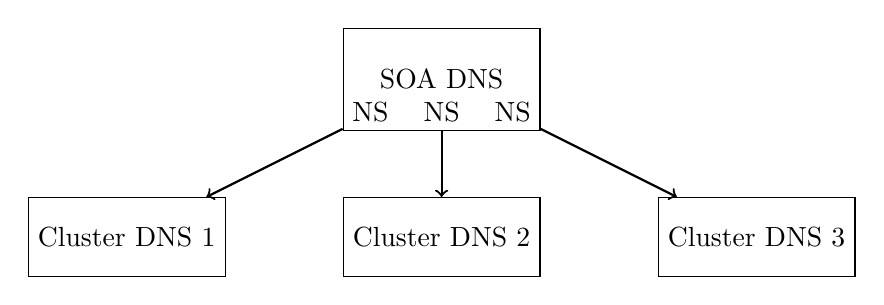
\begin{tikzpicture}[
        node distance = 2cm,
        box/.style = {draw, rectangle, minimum width=2.5cm, minimum height=1cm},
        soabox/.style = {draw, rectangle, minimum width=2.5cm, minimum height=1.3cm},
        arrow/.style = {->, thick}
    ]
    
    % SOA DNS Server at the top
    \node[soabox] (soa) at (0,0) {SOA DNS};
    
    % Cluster DNS servers below
    \node[box] (dns1) at (-4,-2) {Cluster DNS 1};
    \node[box] (dns2) at (0,-2) {Cluster DNS 2};
    \node[box] (dns3) at (4,-2) {Cluster DNS 3};
    
    % Draw arrows
    \draw[arrow] (soa) -- (dns1);
    \draw[arrow] (soa) -- (dns2);
    \draw[arrow] (soa) -- (dns3);
    
    % Add NS record labels to arrows
    \node[above right] at (soa.south west) {NS};
    \node[above] at (soa.south) {NS};
    \node[above left] at (soa.south east) {NS};
    
    \end{tikzpicture}
    \caption{DNS Hierarchy with Multiple Cluster Servers}
    \label{fig:dns-hierarchy}
\end{figure}
\\
\\
Each cluster-level DNS server is responsible for a set of micro clusters, and points to them using AAAA records.
This creates a direct mapping from DNS to services, as seen in Figure \ref{fig:service-dns-mapping}.
In our case each of the cluster-level DNS servers are responsible for micro-clusters of all the services required 
for the application to function. This reduces the need for inter-cluster communication between data centers.
\\
\\
\begin{figure}[h]
    \centering
    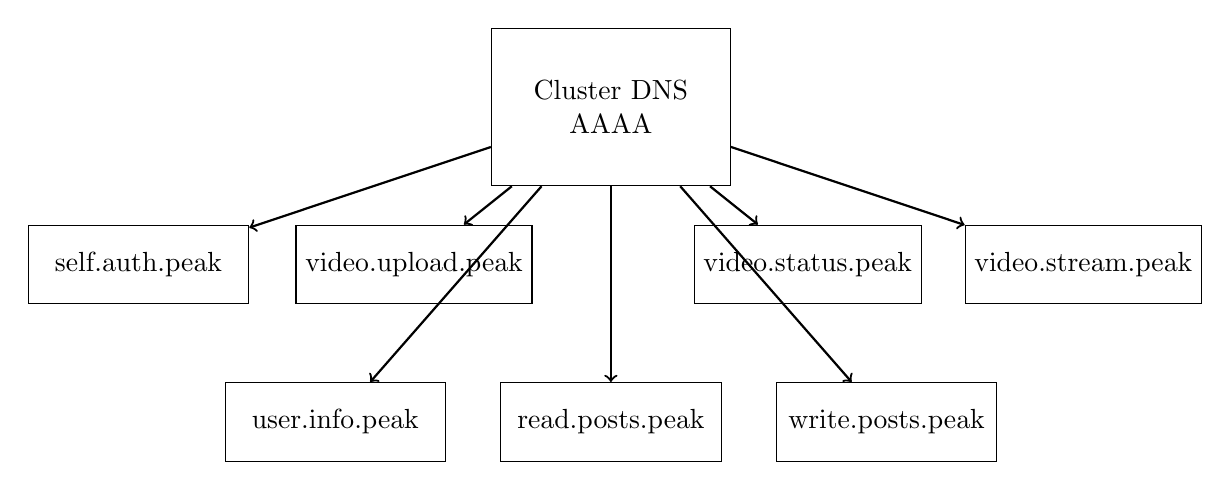
\begin{tikzpicture}[
        node distance = 2cm,
        box/.style = {draw, rectangle, minimum width=2.8cm, minimum height=1cm},
        clusterbox/.style = {draw, rectangle, minimum width=2.8cm, minimum height=2cm},
        arrow/.style = {->, thick}
    ]
    
    % Cluster DNS Server at the top
    \node[clusterbox] (dns) at (0,0) {\parbox{2.8cm}{\centering Cluster DNS \\ AAAA}};
    
    % First row of services
    \node[box] (self) at (-6,-2) {self.auth.peak};
    \node[box] (upload) at (-2.5,-2) {video.upload.peak};
    \node[box] (status) at (2.5,-2) {video.status.peak};
    \node[box] (stream) at (6,-2) {video.stream.peak};
    
    % Second row of services
    \node[box] (info) at (-3.5,-4) {user.info.peak};
    \node[box] (read) at (0,-4) {read.posts.peak};
    \node[box] (write) at (3.5,-4) {write.posts.peak};
    
    % Draw arrows to all services
    \draw[arrow] (dns) -- (self);
    \draw[arrow] (dns) -- (upload);
    \draw[arrow] (dns) -- (status);
    \draw[arrow] (dns) -- (stream);
    \draw[arrow] (dns) -- (info);
    \draw[arrow] (dns) -- (read);
    \draw[arrow] (dns) -- (write);
    
    % Add AAAA labels with more space
    \node[above] at ($(dns)!0.3!(self)$) {};
    \node[above] at ($(dns)!0.3!(upload)$) {};
    \node[above] at ($(dns)!0.3!(status)$) {};
    \node[above] at ($(dns)!0.3!(stream)$) {};
    \node[above] at ($(dns)!0.3!(info)$) {};
    \node[above] at ($(dns)!0.3!(read)$) {};
    \node[above] at ($(dns)!0.3!(write)$) {};
    
    \end{tikzpicture}
    \caption{Direct DNS to Micro Cluster Mapping}
    \label{fig:service-dns-mapping}
\end{figure}
\pagebreak
\printbibliography
\license
\end{document}